\documentclass[11pt,a4paper]{book}
\usepackage[utf8]{inputenc}
\usepackage{amsmath}
\usepackage{amsfonts}
\usepackage{amssymb}
\usepackage{graphicx}
\usepackage{url}
\usepackage{lipsum}
\usepackage{marginnote}
\usepackage{todonotes}

\author{FrontEndART Szoftver Kft.}
\title{User's Guide of the CROSSMINER Advanced Integrated Development Environments Plug-in}
\date{Version 1.0.0.rev0}

\makeatletter
\renewcommand{\maketitle}{
\vspace*{.1\textheight}
\begin{center}
	
\includegraphics[width=.6\textwidth]{pic/CROSSMINER-logo-large.png}
\end{center}
\begin{center}
	\Huge\@title
\end{center}
\vfill
\begin{center}
	\large\@author\\\@date{} $\bullet$ \today
\end{center}
}
\makeatother

\newcommand{\placeholder}[1]{$\left\langle\text{#1}\right\rangle$}

\newcommand{\SHALL}{\colorbox{red!25}{\textsc{shall}}}
\newcommand{\SHOULD}{\colorbox{orange!25}{\textsc{should}}}
\newcommand{\MAY}{\colorbox{cyan!25}{\textsc{may}}}

\newcommand{\status}[1]{\textbf{Status:} #1}
\newcommand{\todom}{\textcolor{gray}{to do}}
\newcommand{\waitingForServer}{\textcolor{red}{waiting for server side implementation}}
\newcommand{\inprogress}{\textcolor{orange}{partially done}}
\newcommand{\done}{\textcolor{green}{done}}

\newcommand{\unknown}{\colorbox{yellow}{???}}

\newcommand{\req}[4][\todom]{\medskip\marginnote{
\includegraphics[width=2.75em]{pic/contract}}\noindent\textbf{\textsf{Requirement #2}} #4  \status{#1}\\\noindent\textit{#3}\bigskip\par}

\begin{document}
	
\begin{titlepage}
	\maketitle
\end{titlepage}

\chapter{Introduction}

The general layout of the development and testing process are shown on Figure~\ref{fig:version}

\begin{figure}[h]
	\centering
	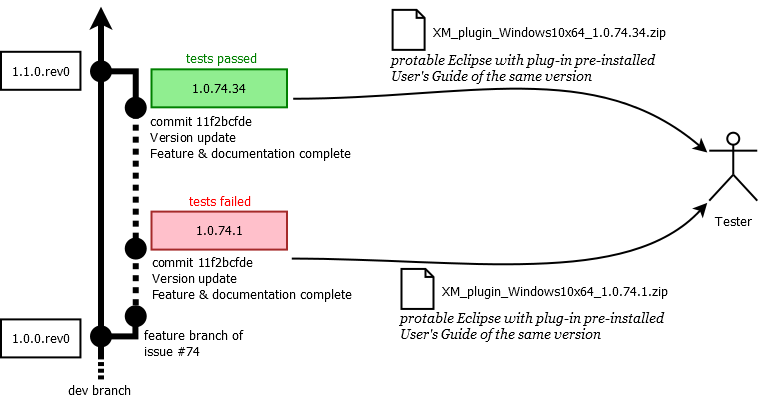
\includegraphics[width=\linewidth]{pic/version.png}
	\caption{Overview of the testing and development process}
	\label{fig:version}
\end{figure}


\section{Versions}
The version number consists of three parts separated by period. It follows the layout \emph{\placeholder{main}.\placeholder{sub}.\placeholder{issue}.rev\placeholder{revision}}. To understand when and how to change these parts please consider the following guide.

\begin{description}
	\item[Increasing main version] Request rights of lead developer or above. It will be increased when the current version are shipped and demonstrated to the (whole) consortium.
	\item[Increasing sub version] Could be changed by any participant. Increase it by one respecting to the current version of the \texttt{dev} branch when a new feature are finished, passed all required tests and merged into the current development version (on \texttt{dev} branch). Reset it to 0 every time main version number increases. 
	\item[Changing issue number] You have to set this part to be equal the identification number of the current issue associated to the feature branch you are on. Set it 0 on non-feature branches.
	\item[Incrementing the revision] Could be changed by any participant. Increment it by one, before you send a new version for testing. It could be the first version containing a testable new feature or any fixes applied due to testers concerns. Reset it to 0 at the beginning of each new feature branch.
\end{description}

There are some additional rules need to consider, partially implicated by the these statements. You have to follow these as well the previous ones.

\begin{description}
	\item[Development versions] Each version on the \texttt{dev} branch should follow this scheme: \emph{\placeholder{main}.\placeholder{sub}.0.rev0}, for example \emph{1.12.0.rev0}.
	\item[Testable versions] Each version sent for testing should follow this scheme: \emph{\placeholder{main}.\placeholder{sub}.\placeholder{current-issue}.rev\placeholder{revision}}, for example \emph{2.23.42.rev11}.
	\item[Version tagging] Each version should be explicitly tagged in the Git repository using the following commands (if your HEAD points to the relevant commit):\\\texttt{git tag \placeholder{version}\\git push origin \placeholder{version}}
	\item[Issue-branch-feature tracibility] Each feature branch has to have a single and unique issue. Do not change (create new) version off the plug-in after merging a branch contains only refactoring without any new features or fixes.
	\item[Tracability of User's Guide] The User's Guide (this document) has to follow the version any version changes. You have to update the guide before you change the version number.
\end{description}

\section{Structure of Releases}

After chancing the version you have to assemble a new release package. By doing so please follow these rules.

\begin{description}
	\item[Naming] Each release package should be named by the following scheme: \emph{XM\_plugin\_\placeholder{operation-system}\_v\placeholder{version}.zip},\\for example \texttt{XM\_plugin\_Windows10x64\_2.23.0.rev0}
	\item[Content] Each release should consist of a single, self-contained compressed folder, containing a portable Eclipse with the plug-in pre-installed.\footnote{Except in the cases, when the goal of testing is installation.}
	\item[Placing Documentation] The relevant version of this document should be placed in the root folder of the compressed package in PDF format.
\end{description}

\section{Testing}

Each feature and function should be tested against expected functionality described in this document. Any discrepancies should be reported.

\begin{description}
	\item[Reporting failed tests] All failed test should be reported using a dedicated issue recorded in the project. \url{https://git.sed.hu/geryxyz/crossminer/issues/new}
	\item[Content of the report] Each report should contain a detailed description of the action and condition of test to be repeatable. You have to specify the concrete version in which the divergence occur and the exact place in this document where the feature was described.
	\item[Goal of testing] As a tester you have to ensure that each features are working as described in this document with reasonable reliability.
\end{description}

\chapter{General features}

In this chapter we present several functions which can not be linked to any single feature.
These embodied an overview about the general principles which interwove the whole plug-in.

\req[\done]{U12}{Able to obtain the API results in JSON format}{\SHALL}
\req[\done]{U13}{Able to use the API over REST}{\SHALL}
\req[\done\todo{done up to date}]{U18}{API is utilised by all UIs (dashboard, IDE plugin)}{\SHALL}

\req[\todom]{U154}{Eclipse users can invoke code recommender via an easy shortcut}{\SHALL}
\req[\todom]{U156}{Eclipse IDE proposes a dedicated view or perspective for recommendations}{\SHALL}
\req[\todom]{U158}{Eclipse IDE plugin can be installed via the Marketplace}{\SHALL}
\req[\done]{U159}{Eclipse IDE plugin can be installed via an update site}{\SHALL}

\req[\todom]{U220}{User and admin documentation is embedded into the UI}{\SHALL}
\req[\done]{U225}{Plugin supports the latest supported release of Eclipse}{\SHALL}

\req[\done\todo{up to date}]{D138}{The CROSSMINER REST API shall use UTF-8 encoding for all kind of data sent or received in text mode.}{\SHALL}

\chapter{Acquire Recommendations}

There are several kind of suggestions and recommendation which could be helpful for the developer during their daily tasks. In this chapter we introduce those features which result some kind of recommendation. One of the main properties is the type of entity which are the subject of the suggestion. To simplify any further discussion our tool only permit recommendation with a single subject type. You can find more details in the following sections.

\req[\waitingForServer\todo{Nothing to do directly on IDE side?}]{U1}{Able to extract the development dependencies of a project}{\SHALL}
\req[\waitingForServer\todo{Nothing to do directly on IDE side?}]{U2}{Able to extract the test dependencies of a project}{\SHALL}
\req[\waitingForServer\todo{Nothing to do directly on IDE side?}]{U3}{Able to extract the runtime dependencies of a project}{\SHALL}

\req[\todom]{U157}{Eclipse IDE proposes filtering options for recommendations}{\SHALL}

\req[\waitingForServer\todo{It is a MAY. Howto: e.g. label recommendation as TEST}]{U223}{Provides recommendations to improve test coverage}{\MAY}

\req[\inprogress]{D75}{Recommendation query shall be initiated from the menu, from context menus, and from the toolbar in the IDE. So the user can easily start working with the recommendations.}{\SHALL}
\req[\todom{} \waitingForServer\todo{Some recommendation types needs to be defined in details (with examples).}]{D76}{The IDE shall use a view to list the code recommendations for the examined project. The view shall provide hierarchical grouping of listed items, filtering by meta-properties, and navigation.}{\SHALL}
\req[\waitingForServer\todo{API needs to be defined. According to L'Aquila the server will receive only a string from a prepared set of options.}]{U167}{CROSSMINER IDE provides the ability for the developer to give feedback on the usefulness of the advices in the given situation}{\SHALL}
\req[\waitingForServer\todo{Not IDE! Needed for U167 and D79}]{D105}{The CROSSMINER REST API should provide an interface that allows the user to report if the answer of query previously returned by the API was inappropriate answer for the query. So the knowledge base gets feedback and can be improved.}{\SHOULD}

\section{Library Based Recommendations}

Recommendation which subject are libraries are called \emph{library based recommendations.}

\req[N/A\todo{WEB Dashboard functionality}]{U4}{Able to warn about superfluous dependencies}{\SHOULD}
\req[N/A\todo{WEB Dashboard functionality}]{U5}{Able to warn about overly precise dependencies}{\SHOULD}

\req[\done]{U81}{Able to identify and list the third-party components used in a project.}{\SHALL}
U81: If we can support all case studies, then the current, client-side maven-based identification is enough.

\req[\inprogress]{D78}{The IDE shall provide an interface to the user, where libraries that match some recommendations are listed with their selected set of details in filterable and sortable form. So the developer can easily compare the libraries and choose those best fit to their expectations.}{\SHALL}
\req[\waitingForServer]{D79}{The IDE should provide the ability to the user to mark a library proposed for a query as ``not appropriate''. This information can help in the improvement of the knowledge base.}{\SHOULD}
\req[\done]{D80}{The IDE shall provide an interface where known information from a single library is shown. This interface can help the user to check details of the library, and reach out for more information through links (e.g. to project home page).}{\SHALL}
\req[\waitingForServer\todo{Not IDE! Needed for D78}]{D100}{The CROSSMINER REST API shall provide an interface that accepts a name and version description and returns the library that is described by them.}{\SHALL}
\req[\done\todo{Not IDE! Needed for D78}]{D101}{The CROSSMINER REST API shall provide an interface that accepts a library and returns detailed information about it (including description, metric values, URLs).}{\SHALL}

\subsection{Searching Additional Libraries}

One sub-type of library based recommendation when the goal of the developer is to find new libraries based on some user specified search criteria.

\req[\waitingForServer]{U172}{CROSSMINER IDE provides developers code templates and example of codes related to the usage of the API of a specific project}{\SHALL}
\todo{U172}U172: A new sub-type of code recommendations is needed to handle code templates.
The KB will send only the changes of the API, which have to be applied on the client side.
The details of the communication must be defined.

\req[\todom{} \waitingForServer\todo{On the IDE side, it is a free text search (with some pre-defined constraints, if needed). Free text search is okay as far as it satisfies all the use cases.}]{D77}{The IDE shall provide an interface, where recommendations against a new (to-be-used-in-the-project) library can be given. So the user can describe features and functionalities they wants to perform using an external library. The user can also give some constraints, e.g. minimal age or users of the library.}{\SHALL}
\req[\inprogress{} \waitingForServer\todo{Not IDE! Needed for D77.}]{D99}{The CROSSMINER REST API shall provide an interface that accepts a description and some filtering constraints and returns a list of libraries that match with the description and fulfil the constraints.}{\SHALL}

\subsection{Searching Similar Libraries}

There are usually some pre-existing selection of libraries which serve as a base to find more relevant API-s. We split these kind of recommendation into two major sub-category: when the pre-existing set of libraries are already installed or not.

\req[\waitingForServer\todo{Not IDE! Needed for U174}]{D102}{The CROSSMINER REST API shall provide an interface that accepts a library, a description and some filtering constraints and returns a list of libraries that match with the description, fulfil the constraints, and can be used as a replacement to the given library.}{\SHALL}

\subsubsection{Suggestion Based on Non-installed Libraries}

\subsubsection{Suggestion Based on Already Installed Libraries}

\req[\waitingForServer\todo{Not IDE! Needed for D81}]{U174}{CROSSMINER IDE provides suggested alternatives to the usage of third-party jar which offer the same range of services as a jar used in current project}{\SHOULD}
\req[\todom{} \waitingForServer]{D81}{The IDE shall provide an interface to the user, where recommendations for replacing a library used in the current project with some alternative libraries can be given. The user can select the library currently used in the project to be replaced and can give further recommendations against the alternatives.}{\SHALL}

\subsection{Handling Changed and Deprecated APIs}

Third party libraries are prone to change and evolution.
To help the developers adapt their project to these changes we defined an other sub-category of recommendations, namely when their goal is to provide information about modified or deprecated interfaces.

\req[\waitingForServer\todo{Not IDE! Needed for U160-162, U164, U168, U169}]{U70}{Able to identify the list of changed third-party API methods from the source code of the third-party API}{\SHALL}
\req[\waitingForServer\todo{Not IDE! Needed for U160-162, U164, U168, U169}]{U71}{Able to identify the list of deprecated third-party API methods from the source code of the third-party API}{\SHALL}
\req[\waitingForServer\todo{Not IDE! Needed for U160-162, U164, U168, U169, U173, U175}]{U72}{Able to determine migration pattern from two (or more) code snippets when one of them uses the old third-party API and the other uses the new third-party API}{\SHALL}

\req[\waitingForServer\todo{Not IDE! Nedded for U160-162, U164, U168, D83-84}]{U80}{Able to detect from the configuration settings if a new version of a used third-party library is available}{\SHALL}
\req[\waitingForServer\todo{Not IDE! Nedded for U160-162, U164, U168, D82-84}]{U130}{Able to identify if the developer is not using the most recent version of a library and provide notification}{\SHALL}

\req[\todom{} \waitingForServer]{U160}{CROSSMINER IDE notifies if a new version of a third-party API used by the project on which the developer is working is available}{\SHALL}
\req[\todom{} \waitingForServer]{U161}{CROSSMINER IDE notifies if a new version of a third-party API used by the project on which the developer is working breaks backward compatibility}{\SHALL}
\req[\todom{} \waitingForServer]{U162}{CROSSMINER IDE is able to offer the use of the newest version of a third-party API utilised in the project}{\MAY}
\req[\inprogress{} \waitingForServer]{U163}{CROSSMINER IDE is able to identify and navigate to those places that became suspicious for changing behaviour after the third-party API version used in the project has changed}{\SHALL}
\req[\inprogress{} \waitingForServer]{U164}{CROSSMINER IDE is able to mark the usage of deprecated third-party APIs in the source code the developer is working on.}{\SHALL}
\req[\todom{} \waitingForServer]{U168}{CROSSMINER IDE is able to notify the developer about third-party API changes that are in design or development phase}{\MAY}
\req[\todom{} \waitingForServer\todo{Summary on IDE side}]{U169}{CROSSMINER IDE is able to provide an overview of the impact of a third-party API change on the project the developer is working on}{\MAY}
\req[\inprogress{} \waitingForServer\todo{Howto: simply insert the received snippet}]{U173}{CROSSMINER IDE assists developers to migrate the current version of a third-party jar to the new version by providing a list of required changes, advices and code templates}{\SHALL}
\req[\inprogress{} \waitingForServer\todo{Howto: simply insert the received snippet}]{U175}{CROSSMINER IDE assists developers to address a deprecated API by proposing an alternative for obtaining the same behaviours of the code}{\SHOULD}

\req[\todom{} \waitingForServer]{D82}{The IDE shall provide the user the ability to initiate library version check. So the user is notified if some libraries used in their project have new versions.}{\SHALL}
\req[\todom{} \waitingForServer]{D83}{The IDE shall perform library version checks on the libraries used in the current project. The check is performed on project load, and only marks the upgradeable libraries.}{\SHALL}
\req[\todom{} \waitingForServer]{D84}{The IDE shall be able to show if a library used in the current project has a new version that satisfies some pre-determined criteria set globally for library upgrades by the user. So the user can see the relevant results of the library upgrade search.}{\SHALL}
\req[\inprogress\todo{ready, up to date}]{D85}{The IDE shall provide an interface where the details of an available library upgrade can be shown. These may include the new version number, release date, number of users, number of bugs, estimated impact of the upgrade, etc.}{\SHALL}
\req[\inprogress{}\todo{ready, up to date}]{D86}{The IDE should provide the ability to initiate a library upgrade that marks all those places in the source code that needs rework due to the change of the library version.}{\SHOULD}
\req[\inprogress{}\todo{ready, up to date}]{D88}{The IDE may perform the steps of a library upgrade autonomously (if the user requested the upgrade).}{\MAY}
\req[\inprogress{} \waitingForServer\todo{Not IDE!}]{D103}{The CROSSMINER REST API shall provide an interface that accepts a library and filters, and returns a list of versions available for that library and match the filters.}{\SHALL}
\req[\waitingForServer\todo{Not IDE! Needed for D86, D88}]{D104}{The CROSSMINER REST API shall provide an interface that accepts a library and two versions, and returns the differences between these library versions. Differences include removed, deprecated, changed, new API elements, and API elements with changed behaviour.}{\SHALL}

\section{Source Code Based Recommendations}

In this section we elaborate features related to those recommendation which subject entities are present in the source code of the project under development. They usually retrieve some code chunk, which could be annotated to ease further understanding.

\req[\inprogress\todo{Not IDE! Needed for U170-171...}]{U73}{Able to identify the part of the API that the developer is currently using to provide code snippets in relation with current development activity}{\SHALL}
\req[\inprogress{} \waitingForServer\todo{no data for ``as suspicious''}]{U170}{CROSSMINER IDE provides the ability for the developer to ask recommendations for a code chunk previously marked by the CROSSMINER IDE as suspicious}{\SHOULD}
\req[\done]{U171}{CROSSMINER IDE provides the ability for the developer to ask recommendation for an arbitrary code chunk or code element}{\SHOULD}

\req[\inprogress]{D92}{The IDE should provide the ability to the user to select a code snippet or a file and ask for code recommendations for it. So the user can check whether there is a better practice to solve her problem.}{\SHOULD}
\todo{D92}Code recommendations for arbitrary code is enough.
The CROSSMINER API should provide a point where context information (the whole project?) can also be uploaded (Davide said that it already exists).
The content and form of it must be discussed.

\req[\inprogress]{D93}{The IDE should be able to show recommendations assigned with code elements. So the user can see what the knowledge base suggested for a code snippet.}{\SHOULD}
\todo{D93}Code recommendations for arbitrary code can be enough, but the CROSSMINER API can also provide a point for code element recommendations.
The CROSSMINER API should provide a point where context information (the whole project?) can also be uploaded (Davide said that it already exists).
The content and form of it must be discussed.

\req[\waitingForServer\todo{Not IDE! Needed for U170-171, D91-94}]{D107}{The CROSSMINER REST API may provide an interface that accepts code snippets and library context, and returns recommendations on how to improve that part of the code.}{\MAY}

\subsection{Retrieving Suggested Code Snippets}

Based on the current development context, our plug-in is able to yield a set of source code snippets (code chunks), which could be useful to implement or to understand various features.

\req[\done\todo{done, up to date}]{D91}{The IDE may insert a recommendation in the code if the user accepts it and requested it on a code position.}{\MAY}
\req[\inprogress{} \waitingForServer\todo{``IDE replaces ...'' will probably not be implemented, unless the server gives proper recommendations}]{D94}{The IDE may be able to process recommendations and perform code migration autonomously. So the user can point to a recommendation and the IDE replaces the old code to the new one.}{\MAY}
\req[\waitingForServer\todo{Not IDE! Needed for U170-171, D91-94}]{D106}{The CROSSMINER REST API may provide an interface that accepts a list of libraries and a description and returns recommendations about how to implement the described functionality using the given libraries.}{\MAY}

\section{Text Based Recommendations}

Finally there are tons of documentation and discussion available for various topics, which could be useful for the developers. Those recommendations which yield some natural language documents (or reference to them) are called \emph{text based recommendations.}

\subsection{API Usage}

Developers could use these recommendation to get more information about the features and their usage of a 3rd part API, for example official pages, documentations, and examples.

\req[\todom{} \todo{It is a MAY. Davide said that the API is prepared for sending context-data}\waitingForServer]{D89}{The IDE may provide an interface where description of a feature to be implemented and libraries that should be used to implement it can be given. So the user can ask for recommendations how to implement features using specific libraries.}{\MAY}
\req[\todom{} \todo{It is a MAY. Davide said that the API is prepared for sending context-data}\waitingForServer]{D90}{The IDE may provide an interface to show recommendations on how to implement a feature using some specific libraries.}{\MAY}

\subsection{Handling API changes}

There several forum threads and change reports, which could ease the migration between different versions of the same library.

\req[\todom{} \waitingForServer]{U165}{CROSSMINER IDE offers a list of community discussion forums concerning the use of a changed third-party API element}{\SHOULD}
\req[\todom{} \waitingForServer]{U166}{CROSSMINER IDE offers code examples for deprecated third-party API usage points}{\SHOULD}
\req[\todom{} \waitingForServer]{D87}{The IDE shall provide an interface that explains the steps of how to upgrade a library used in the project to a new version.}{\SHALL}

\subsection{Inspecting Code Chunk Related Q\&A Posts}

Also there are some discussions about how to implement a function using a specific features or a set of libraries. The recommendations which present these documents (posts and blog entries) are represent an other subclass of text based recommendations.

\chapter{User Activity Monitoring}

\req[\todom\todo{Not specific to IDE}]{U176}{There is a strict and public strategy regarding privacy and data}{\SHALL}
\req[\todom{} \waitingForServer\todo{Not specific to IDE}]{U177}{Users cannot be identified from monitoring data}{\SHALL}
\req[\inprogress]{U178}{Monitoring is able to identify testing activities}{\SHOULD}
\req[\done]{U179}{Monitoring is able to identify development activities}{\SHOULD}
\req[\unknown\todo{This needs to be clarified}]{U180}{Monitoring is able to identify errors in IDE}{\SHOULD}
\req[\inprogress]{U181}{Monitoring records the time the developer works on a given file/code element/line}{\SHOULD}

\req[\inprogress]{U218}{All metrics are documented, motivated, possibly with references}{\SHALL}

\req[\todom\todo{Details needs to be defined. Search expressions come only from searches in the plug-in.}]{D96}{The IDE shall recognize, compute, and extract the following user activities, metrics, or information: frequent search expression.}{\SHALL}
\req[\inprogress\todo{Search patterns come only from searches in the plug-in.}]{D97}{The IDE should recognize, compute, and extract the following user activities, metrics, or information: project or file open, manipulation, close, program execution, test execution, user search patterns, working time on a file.}{\SHOULD}
\req[\waitingForServer\todo{Not IDE! Needed for U176-181, D96-98}]{D108}{The CROSSMINER REST API shall provide an interface that accepts developer activity data. So the CROSSMINER can build this information in the knowledge base.}{\SHALL}

\section{Retrieving Process Metrics via \textsc{crossminer} Web-based Dashboard}

You are able to inspect any computed process metrics for your project by using the relevant features of CROSSMINER Web-based Dashboard.

\section{Plug-in Side Debugging Features}

In the case of unexpected errors during the user activity monitoring, you are able to check the value of the process metrics and some relevant meta-data about the underlying database on the client side. To do this please activate some of the plug-in side debugging features. Please note that these are only available in the debug version of the plug-in. 

\section{Server Side Debugging Features}

There are ways to access the raw data, stored at the server side. To do this you have to execute the following REST API calls. You could use your preferred REST client, but for illustration purposes we will use Postman\footnote{\url{https://www.getpostman.com/}}

\req[\todom]{D98}{The IDE shall be able to send developer activity data (as controlled by the user settings) to the CROSSMINER server.}{\SHALL}

\chapter{Settings and Customization}

\req[\todom\todo{Not IDE!}]{U155}{Eclipse users can easily deactivate the analysis}{\SHALL}

\section{Integration Related Settings}

\req[\inprogress]{D74}{The IDE shall provide a settings interface to the user, where the different properties of the CROSSMINER IDE plugin (like server address and port, global settings for recommendation queries, etc.) can be checked and changed. So the user can configure the plugin.}{\SHALL}

\section{Process Metric Related Settings}

\req[\todom]{U182}{Monitoring of developer activity can be disabled by the developer}{\SHALL}
\req[\todom]{U183}{Types of data collected from monitoring are transparent to the developer}{\SHALL}
\req[\todom]{D95}{The IDE shall provide full control over the collected and transferred user activity monitoring data. So the user can allow or deny the collection and/or anonymised transfer of the activity data collected from their session.}{\SHALL}

\end{document}
